\documentclass[aspectratio=43,12pt]{beamer}

\setbeamersize{text margin left=1cm,text margin right=-4.5cm}

% Theme works only with a 4:3 aspect ratio
\usetheme{CSCS}

% define footer text
\newcommand{\footlinetext}{\arbor{}}

% Select the image for the title page
\newcommand{\picturetitle}{cscs_images/image3.pdf}
\newcommand{\arbor}{Arbor}

\newcommand{\subheading}[1]{{\large #1}}
\newcommand{\TODO}[1]{\textcolor{red}{TODO: \bf #1}}

% Please use the predifined colors:
% cscsred, cscsgrey, cscsgreen, cscsblue, cscsbrown, cscspurple, cscsyellow, cscsblack, cscswhite

% colour rebel!
\definecolor{light-grey}{gray}{0.6}

\author{Alexander Peyser, FZ-J \& Sam Yates, CSCS}
\title{\arbor}
\subtitle{A new multi-compartment neuron simulator}
\date{\today}

\begin{document}

% --
\addtolength{\headsep}{-0.3cm}
\setbeamertemplate{footline}{}
\begin{frame}[shrink]
\frametitle{\hspace{-0.5cm}\raisebox{-0.5\height}{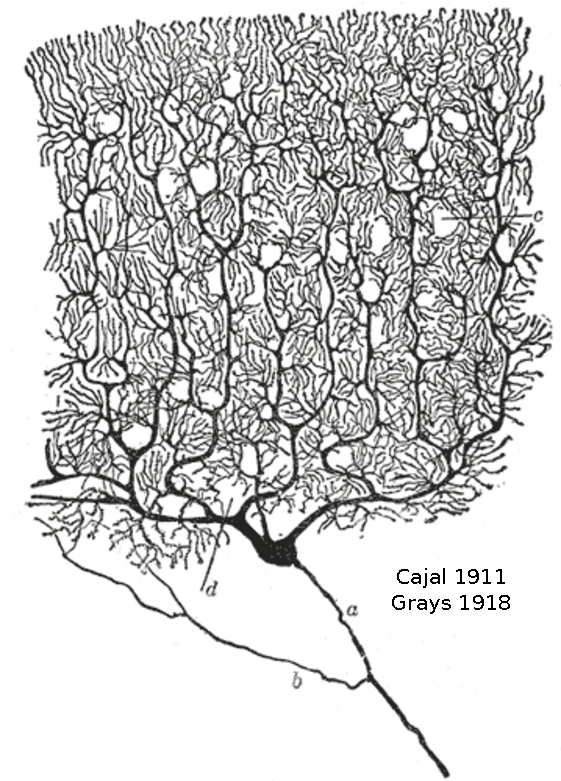
\includegraphics[width=1cm]{cajal}}\arbor}
\vspace{0.2\baselineskip}
\arbor{} (\url{https://github.com/arbor-sim/arbor}) is a \\\hspace{1em}\textcolor{cscsblue}{new} library for multi-compartment neuronal network simulation.
\setlength\leftmargini{1.2em}
\begin{itemize}%[leftmargin=0pt]
\item \textcolor{cscsblue}{Open source} --- all code, documentation and bug-tracking is public
\item \textcolor{cscsblue}{Optimized} for HPC systems by HPC centers to ensure that\\\hspace{1em} all HPC infrastructure can support state of the art simulations
  \begin{itemize}
  \item Performance portable
    \begin{itemize}
    \item Optimized for NVIDIA GPUs, Intel CPUs and Intel KNL
    \item Modular design for new backends\\\hspace{1em} such as ARM SVE (EuroHPC) and AMD GPUs
    \end{itemize}
        
  \item Scales for foreseeable node and cluster architectures.
  \item Modern C++ design: lean and modular
  \end{itemize}
  
\item \textcolor{cscsblue}{Easy to integrate} into existing workflows
  \begin{itemize}
  \item configurable to share resources on a system
  \item native Python interface
  \item designed to couple with other simulators, analysis tools\\\hspace{1em} and in-situ visualization
  \end{itemize}
\end{itemize}
\vfill
\end{frame}

\begin{frame}[shrink]
\frametitle{\hspace{-0.5cm}\raisebox{-0.5\height}{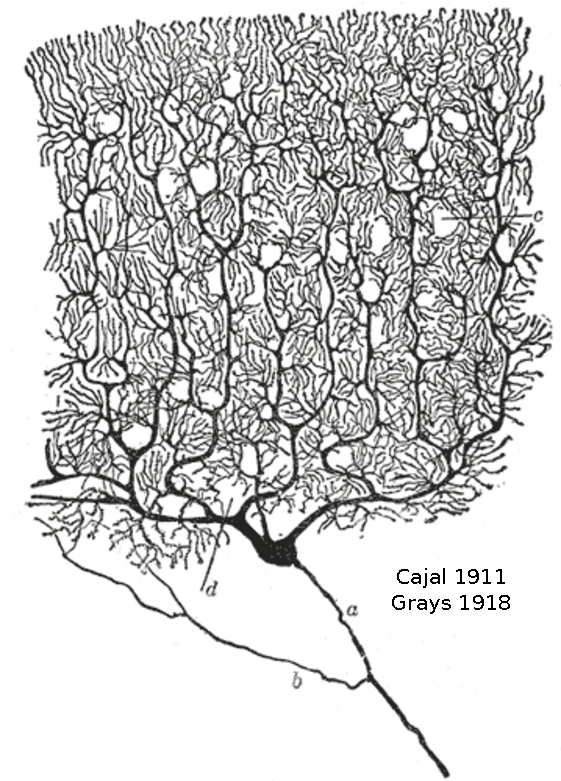
\includegraphics[width=1cm]{cajal}}\arbor}
\vspace{0.2\baselineskip}
\textcolor{cscsblue}{Completed features}
\begin{itemize}
\item Finite-volume based discretization
\item Distributed model instantiation
\item Spike and voltage trace output
\item x66 multi-core and Intel KNL support
\item GPU support
\item Synapse and ion-channel descriptions in NMODL
\item Unit and validation testing suite
\end{itemize}

\textcolor{cscsblue}{Available soon}
\begin{itemize}
\item Python front-end branch
\item Live on-line spike exchange with NEST as part of a\\multiscale environment with TVB and in-situ visualization
\item Benchmark suite including NEST and NEURON
\item Efficient gap junction schemes
\end{itemize}
\vfill
\end{frame}

\end{document}
